\chapter{Adaptasi Tumbuhan dan Keplastisan Fenotipe}\label{ch:b2:plant-plasticity}

Dua helai daun dari pohon ek yang sama: yang dari puncak tajuknya
kecil, tebal, dan liat, sedangkan yang dari bagian dalam yang ternaung
tiga kali lebih lebar dan setipis kertas. Sebuah semai pohon ek yang
sama di bawah kanopi yang rapat tumbuh jangkung dan kurus; saudaranya
di sebuah lapangan terbuka tetap pendek dan kekar. Tak satu pun
perbedaan itu bersifat genetik. Sebatang tumbuhan tidak dapat berjalan
ke tempat yang lebih baik, maka ia membangun dirinya agar pas dengan
tempat yang ia punya: ia mengindra cahaya, gravitasi, sentuhan, air,
garam, dan dingin, lalu ia membengkok, menebal, memanjang, menutup
porinya, atau mengeraskan selnya sesuai dengan itu. Bab ini membahas
keplastisan itu --- bagaimana sebatang tumbuhan membaca sekelilingnya
dan apa yang ia lakukan terhadapnya --- serta \omterm{def:b2:plant-plasticity:plasticity}{adaptasi} yang terwariskan
yang dengannya garis keturunan telah menyesuaikan dirinya dengan gurun,
naungan, garam, dan embun beku.

\section{Keplastisan dan batasnya}

\begin{definition}[Keplastisan fenotipe dan norma reaksi]\label{def:b2:plant-plasticity:plasticity}
\index{keplastisan fenotipe}\index{norma reaksi}\index{aklimasi}\index{adaptasi}
\emph{Keplastisan \omterm{def:b2:meiosis-heredity:vocabulary}{fenotipe}} adalah kemampuan satu \omterm{def:b2:meiosis-heredity:vocabulary}{genotipe} untuk
menghasilkan \omterm{def:b2:meiosis-heredity:vocabulary}{fenotipe} yang berbeda-beda di lingkungan yang
berbeda-beda. \emph{Norma reaksi} sebuah \omterm{def:b2:meiosis-heredity:vocabulary}{genotipe} adalah kurva
\omterm{def:b2:meiosis-heredity:vocabulary}{fenotipenya} terhadap sebuah peubah lingkungan --- ketebalan daun
terhadap cahaya, panjang batang terhadap suhu; \omterm{def:b2:meiosis-heredity:vocabulary}{genotipe} berbeda-beda
dalam normanya, dan perbedaannya terwariskan sekalipun keplastisannya
sendiri tidak. \emph{Aklimasi} adalah bentuknya yang faali dan dapat
balik: sehelai daun yang menebalkan kutikulanya dalam sepekan yang
kering, sebuah sel yang membuat zat antibeku pada musim gugur.
\emph{Adaptasi}, dalam pengertian evolusioner, adalah kecocokan sebuah
garis keturunan dengan habitatnya yang terwariskan dan terseleksi
selama banyak generasi; sebatang kaktus teradaptasi dengan kekeringan,
sedangkan sebatang buncis beraklimasi dengan sebuah masa kering.
Tumbuhan lebih plastis daripada hewan karena ia modular dan tak
tertentu (\cref{ch:b2:plant-meristems}): daun berikutnya dapat dibangun
berbeda dari daun sebelumnya, dan hidup yang terpaku membuat
keplastisan menjadi satu-satunya cara untuk berpindah.
\end{definition}

\begin{omfigure}
\begin{tikzpicture}
\begin{axis}[
  width=0.72\linewidth, height=5.4cm,
  axis x line=bottom, axis y line=left,
  xmin=0, xmax=100, ymin=0, ymax=1.2,
  xlabel={cahaya (\% dari matahari penuh)}, ylabel={ketebalan daun (nisbi)},
  xlabel style={font=\small, at={(axis description cs:0.5,-0.13)}, anchor=north},
  ylabel style={font=\small},
  tick label style={font=\small}, xtick={0,25,50,75,100}, ytick={0,0.5,1},
  legend style={font=\scriptsize, at={(0.97,0.08)}, anchor=south east, draw=none},
  clip=false,
]
\addplot[very thick, omDef, domain=2:100, samples=60] {0.35 + 0.65*(1-exp(-x/30))};
\addlegendentry{genotipe 1: sebatang ek yang plastis}
\addplot[very thick, omThm, domain=2:100, samples=60] {0.55 + 0.2*(1-exp(-x/30))};
\addlegendentry{genotipe 2: satu yang kurang plastis}
\end{axis}
\end{tikzpicture}

{\small Dua \omterm{def:b2:plant-plasticity:plasticity}{norma reaksi}. Tiap \omterm{def:b2:meiosis-heredity:vocabulary}{genotipe} membuat daun yang lebih tebal
pada cahaya yang lebih banyak; kemiringan kurvanya --- keplastisannya
--- itu sendiri merupakan sifat yang terwariskan, dan kedua \omterm{def:b2:meiosis-heredity:vocabulary}{genotipenya}
berbeda dalam hal itu.}
\end{omfigure}

\begin{proposition}[Daun matahari dan daun naungan]\label{prop:b2:plant-plasticity:sunshade}
\index{daun matahari}\index{daun naungan}
Sehelai daun yang berkembang di bawah matahari penuh berukuran kecil,
tebal, dengan dua atau tiga lapis sel tiang, banyak stoma, kutikula
yang tebal, kepekatan enzim pemfiksasi karbon yang tinggi, dan laju
fotosintesis maksimal yang tinggi; sehelai daun tumbuhan yang sama yang
berkembang di dalam naungan berukuran lebar, tipis, dengan satu lapis
sel tiang, lebih banyak klorofil tiap satuan massa, laju respirasi yang
rendah, dan titik kompensasi cahaya yang rendah. \omterm{prop:b2:plant-plasticity:sunshade}{Daun naungannya}
dibangun untuk memanen tiap foton dengan ongkos yang sekecil mungkin,
sedangkan \omterm{prop:b2:plant-plasticity:sunshade}{daun mataharinya} untuk memakai banjir foton tanpa kepanasan
atau layu. Keputusannya diambil ketika daunnya masih berupa primordium,
dari cahaya --- dan terutama warna cahayanya --- yang mencapai
tunasnya; sehelai daun yang masak tidak dapat membangun ulang dirinya,
dan itulah sebabnya tumbuhan yang dipindahkan dari naungan ke matahari
hangus sampai ia telah membuat daun yang baru.
\end{proposition}

\begin{omfigure}
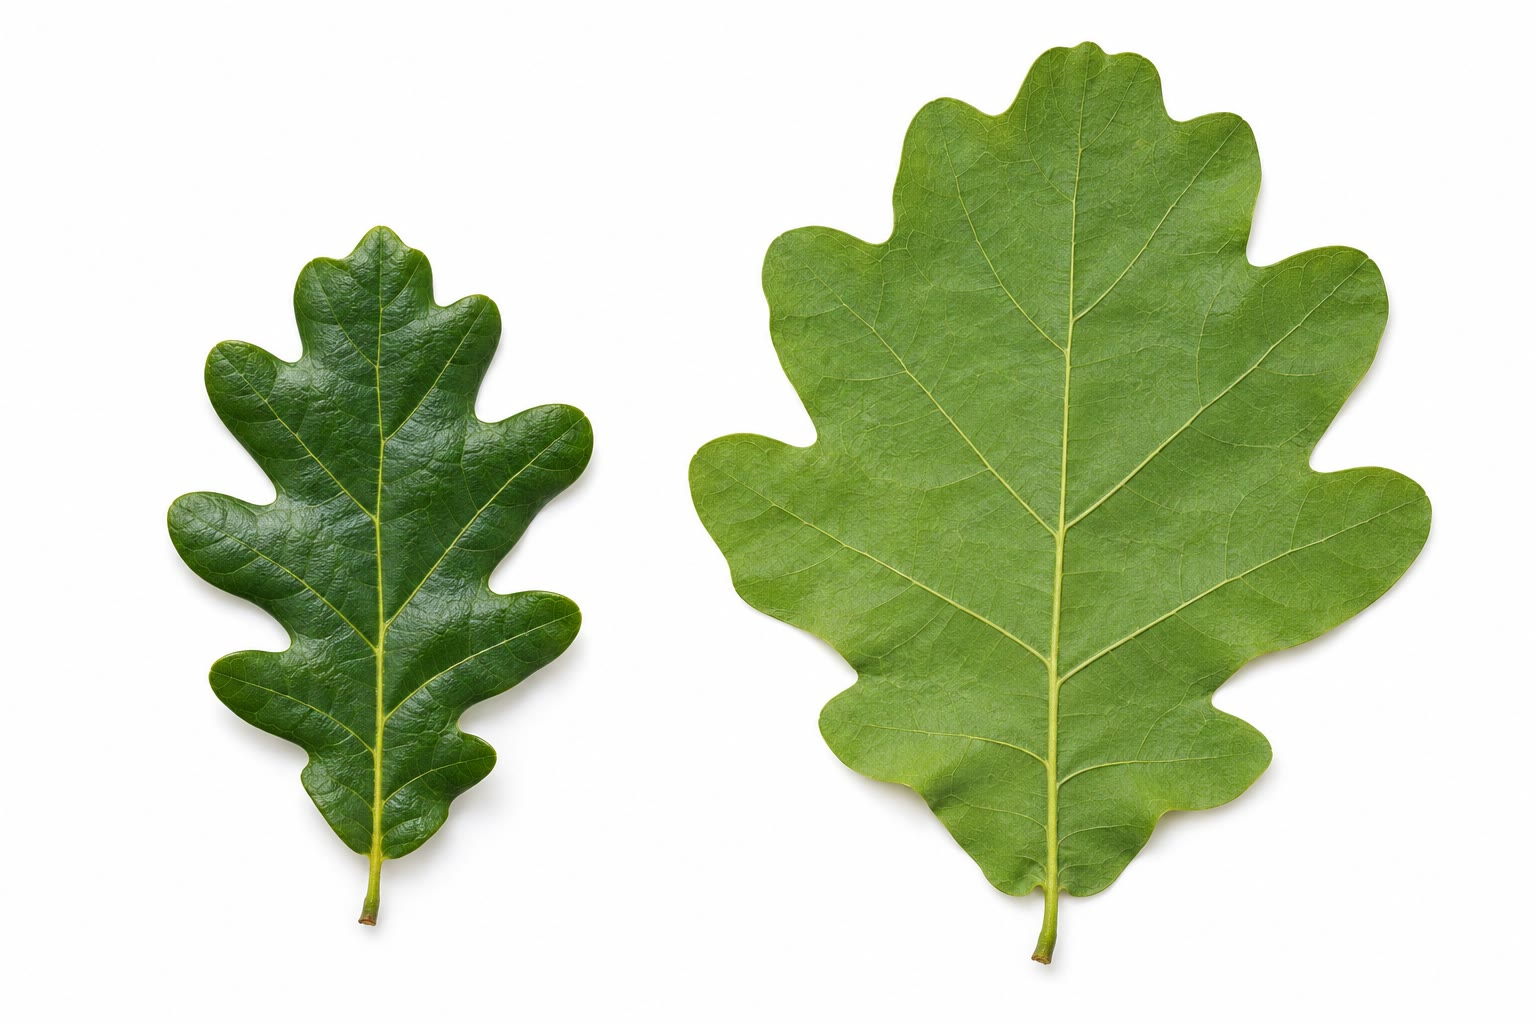
\includegraphics[width=0.55\linewidth]{images/book4/ai/b4-15-sun-shade-leaves.jpg}

{\small Sehelai \omterm{prop:b2:plant-plasticity:sunshade}{daun matahari} dan sehelai \omterm{prop:b2:plant-plasticity:sunshade}{daun naungan} dari satu pohon
ek: \omterm{def:b2:meiosis-heredity:vocabulary}{genotipe} yang sama, cahaya yang berbeda, daun yang berbeda.}
\end{omfigure}

\section{Membaca cahayanya}

\begin{theorem}[Fitokrom sebagai pengukur mutu cahaya]\label{thm:b2:plant-plasticity:phytochrome}
\index{fitokrom}\index{nisbah merah:merah jauh}\index{penghindaran naungan}
Fitokrom hadir dalam dua bentuk: $P_r$, yang menyerap cahaya merah
(\qty{660}{nm}) lalu diubah menjadi $P_{fr}$, dan $P_{fr}$, yang
menyerap merah jauh (\qty{730}{nm}) lalu diubah kembali --- dan
$P_{fr}$-lah yang bekerja. Di dalam cahaya yang menerus kedua
pengubahannya berimbang pada sebuah \emph{kesetimbangan foto} yang
kedudukannya hanya bergantung pada nisbah merah terhadap merah jauh di
dalam cahayanya:
\[
\varphi = \frac{P_{fr}}{P_{r} + P_{fr}} = \frac{R}{R + a\,FR},
\]
dengan $R$ dan $FR$ adalah rapat fluks foton pada kedua pita itu dan
$a$ sebuah tetapan pigmennya ($a \approx 0.77$). Cahaya matahari
memiliki $R{:}FR \approx 1.15$, sehingga $\varphi \approx 0.6$; cahaya
yang tersaring lewat dedaunan, yang menyerap merah dan meneruskan merah
jauh, memiliki $R{:}FR
\approx 0.2$ dan $\varphi \approx 0.2$. Nilai
$\varphi$ yang rendah memberi tahu sebatang tumbuhan bahwa ia berada di
bawah atau di samping tumbuhan lain sebelum ia benar-benar ternaung ---
merah jauh yang terpantul dari tetangganya terdeteksi pada sisi yang
menghadap tetangganya --- dan ia menanggapinya dengan \emph{sindrom
\omterm{thm:b2:plant-plasticity:phytochrome}{penghindaran naungan}}: pemanjangan batang yang lebih cepat, tangkai
daun yang lebih panjang, daun yang ditegakkan ke atas, percabangan yang
lebih sedikit, pembungaan yang lebih awal. Sebuah semai di dalam kanopi
yang rapat melipatduakan laju pemanjangannya.
\end{theorem}
\begin{proof}
Misalkan $k_1 R$ adalah tetapan laju bagi $P_r \to P_{fr}$ (sebanding
dengan fluks merahnya) dan $k_2\,FR$ tetapan laju bagi $P_{fr} \to P_r$.
Pada kesetimbangan $k_1 R\,P_r = k_2\,FR\,P_{fr}$, sehingga $P_{fr}/P_r = k_1 R/
(k_2 FR)$ dan $\varphi = P_{fr}/(P_r + P_{fr}) = R/(R + a\,FR)$ dengan
$a = k_2/k_1$. (Kedua bentuknya sedikit banyak menyerap pada kedua
pitanya, dan tetapan $a$ menyerap hal itu; bentuk hasilnya tidak
berubah.) Dengan $a = 0.77$: $1.15/(1.15 + 0.77) = 0.60$; $0.2/(0.2 + 0.77) = 0.21$.
\end{proof}

\begin{omfigure}
\begin{tikzpicture}
\begin{axis}[
  width=0.7\linewidth, height=5.2cm,
  axis x line=bottom, axis y line=left,
  xmin=0, xmax=1.4, ymin=0, ymax=0.8,
  xlabel={nisbah merah : merah jauh cahayanya}, ylabel={$\varphi = P_{fr}/P_{\text{total}}$},
  xlabel style={font=\small, at={(axis description cs:0.5,-0.13)}, anchor=north},
  ylabel style={font=\small},
  tick label style={font=\small}, xtick={0,0.2,0.6,1.15}, ytick={0,0.2,0.4,0.6},
  clip=false,
]
\addplot[very thick, omDef, domain=0:1.4, samples=60] {x/(x+0.77)};
\draw[dashed, gray] (axis cs:1.15,0) -- (axis cs:1.15,0.6) -- (axis cs:0,0.6); \node[font=\scriptsize, anchor=south west] at (axis cs:1.15,0.6) {matahari terbuka};
\draw[dashed, gray] (axis cs:0.2,0) -- (axis cs:0.2,0.21) -- (axis cs:0,0.21); \node[font=\scriptsize, anchor=west] at (axis cs:0.25,0.15) {di bawah sebuah kanopi};
\end{axis}
\end{tikzpicture}

{\small Kesetimbangan foto fitokrom terhadap nisbah merah terhadap
merah jauh. Cahaya matahari menahan sebagian besar pigmennya dalam
bentuk yang aktif; cahaya yang tersaring dedaunan menahannya sebagian
besar tak aktif, dan tumbuhannya membaca perbedaannya sebagai
tetangga.}
\end{omfigure}

\begin{proposition}[Fototropisme]\label{prop:b2:plant-plasticity:phototropism}
\index{fototropisme}\index{tropisme}\index{hipotesis Cholodny--Went}
Sebuah \emph{tropisme} adalah gerak tumbuh yang diarahkan oleh sebuah
rangsangan berarah. Pada \emph{fototropisme} sebatang pucuk membengkok
menuju cahaya biru: cahayanya diindra di ujungnya oleh sebuah reseptor
cahaya biru (fototropin), auksin yang turun dari ujungnya dialihkan ke
sisi yang ternaung --- pengangkutnya berpindah ke membran lateralnya
--- dan sisi yang ternaung, yang menerima lebih banyak auksin,
memanjang lebih cepat daripada sisi yang tersinari, sehingga pucuknya
melengkung menuju cahayanya. Pembengkokannya adalah pertumbuhan yang
tak sama, bukan sebuah otot: ia hanya terjadi di \omterm{prop:b2:plant-meristems:ram}{zona pemanjangannya},
memakan waktu satu atau dua jam, dan tidak dapat balik. Akar, yang di
dalamnya kelebihan auksin yang sama justru \emph{menghambat}
pemanjangan, membengkok menjauh.
\end{proposition}
\begin{proof}[Bukti eksperimental]
Darwin (1880) menunjukkan dengan koleoptil rumput bahwa ujungnya
mengindra cahayanya dan zona di bawahnya membengkok: menudungi ujungnya
dengan tudung yang tak tembus cahaya meniadakan pembengkokannya,
menudungi pangkalnya dengan sebuah tabung tidak, dan sebuah tudung yang
bening membiarkannya utuh. Boysen-Jensen (1913) memotong ujungnya lalu
memasangnya kembali dengan sekeping gelatin di antaranya: pembengkokannya
bertahan, jadi isyaratnya adalah sebuah zat yang dapat berdifusi;
selembar mika yang disisipkan pada sisi yang ternaung menghalanginya,
pada sisi yang tersinari tidak, jadi zatnya berjalan turun di sisi yang
ternaung. Went (1928) mengumpulkan zatnya dalam agar dari ujung yang
dipotong dan menemukan bahwa sekeping agar yang diletakkan menepi pada
sebatang koleoptil tanpa ujung di dalam gelap membuatnya membengkok
menjauhi kepingnya --- dengan sudut yang sebanding dengan jumlahnya ---
dan, dengan mengumpulkan agar dari kedua belahan sebuah ujung yang
disinari dari satu sisi, menemukan kira-kira dua pertiga auksinnya pada
sisi yang ternaung dan sepertiga pada sisi yang tersinari (Briggs, 1957,
dengan metode yang lebih baik). Pengalihan lateral sebuah hormon
pertumbuhan itulah \omterm{prop:b2:plant-plasticity:phototropism}{hipotesis Cholodny--Went}, dan ia telah bertahan.
\end{proof}

\begin{omfigure}
\begin{tikzpicture}[every node/.style={font=\scriptsize}, >=stealth]
  \foreach \x/\lab/\cap/\bend in {0/{utuh:\\membengkok}/0/1, 2.6/{ujung ditudungi:\\tak membengkok}/1/0, 5.2/{pangkal ditudungi:\\membengkok}/2/1, 7.8/{ujung dipotong:\\tak membengkok}/3/0, 10.4/{ujung di atas gelatin:\\membengkok}/4/1} {
    \begin{scope}[xshift=\x cm]
      \fill[omExo!30] (-0.7,0) rectangle (0.7,0.2);
      \ifnum\bend=1
        \draw[very thick, omExo!70!black] (0,0.2) -- (0,1.6) .. controls (0,2.3) and (0.5,2.6) .. (0.9,2.8);
      \else
        \draw[very thick, omExo!70!black] (0,0.2) -- (0,3.0);
      \fi
      \ifnum\cap=1 \fill[black] (-0.2,2.7) rectangle (0.2,3.1); \fi
      \ifnum\cap=2 \fill[black] (-0.2,0.2) rectangle (0.2,1.5); \fi
      \ifnum\cap=3 \draw[thick] (-0.3,2.6) -- (0.3,2.6); \fi
      \ifnum\cap=4 \fill[omDef!35] (-0.2,2.55) rectangle (0.2,2.75); \draw[very thick, omExo!70!black] (0.55,2.75) -- (0.9,3.1); \fi
      \node[below, align=center] at (0,-0.15) {\lab};
    \end{scope}
  }
  \node[anchor=east, align=right, omProp!80!black] at (-1.0,2.2) {cahaya dari\\sebelah kanan $\to$};
\end{tikzpicture}

{\small Percobaan koleoptilnya. Darwin: ujungnya mengindra cahayanya
dan daerah di bawahnya membengkok; menudungi ujungnya menghentikannya,
melindungi pangkalnya tidak. Boysen-Jensen: isyaratnya melintasi
sekeping gelatin --- ia adalah sebuah zat.}
\end{omfigure}

\begin{omfigure}
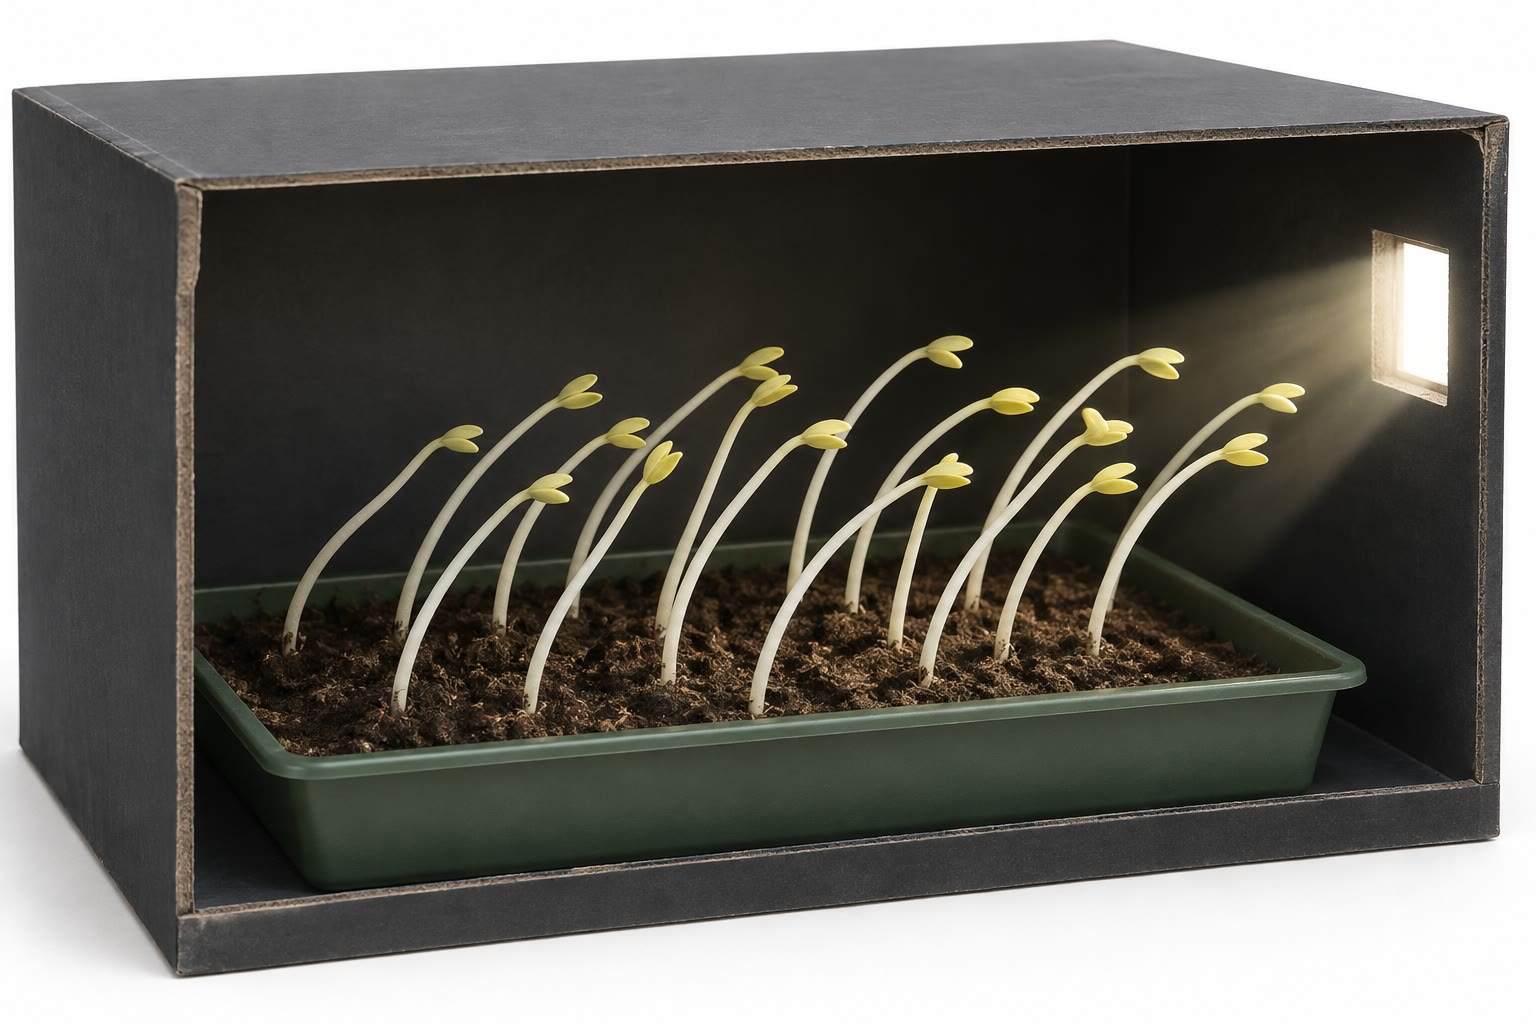
\includegraphics[width=0.55\linewidth]{images/book4/ai/b4-15-phototropism.jpg}

{\small Semai di dalam sebuah kotak dengan satu jendela: semuanya
membengkok menuju cahayanya, dengan tumbuh lebih cepat pada sisi yang
membelakanginya.}
\end{omfigure}

\begin{theorem}[Seberapa jauh sebatang batang membengkok]\label{thm:b2:plant-plasticity:bend}
Jika sisi sebatang batang yang ternaung, yang bergaris tengah $d$,
memanjang dengan jumlah nisbi $\varepsilon_s$ dan sisi yang tersinari
dengan $\varepsilon_l$ sepanjang sebuah zona tumbuh yang panjangnya
$L$, zona itu melengkung sebesar sudut
\[
\theta = \frac{L\,(\varepsilon_s - \varepsilon_l)}{d}
\]
(dalam radian). Sebatang koleoptil yang tumbuh \qty{5}{\%} tiap jam
sepanjang zona \qty{10}{mm} dan bergaris tengah \qty{1}{mm}, dengan
auksin yang terbagi $65 : 35$ sehingga kedua sisinya tumbuh $1.3$ dan
$0.7$ kali reratanya, membengkok dalam tiga jam sebesar $\theta = 10\times(0.195 - 0.105)/1 =
0.9$ radian, kira-kira \qty{50}{\degree}. Pembengkokannya tidak
memerlukan mekanisme yang baru: pertumbuhan biasa pada
\cref{ch:b2:plant-meristems}, yang dibuat tak sama pada kedua sisinya,
sudah memadai.
\end{theorem}
\begin{proof}
Kedua sisi zonanya menjadi busur berjari-jari $\rho + d/2$ dan
$\rho - d/2$ yang mengapit sudut $\theta$ yang sama, yang panjangnya $L(1 +
\varepsilon_s)$ dan $L(1 + \varepsilon_l)$; selisihnya adalah
$\theta d$, sehingga $\theta = L(\varepsilon_s - \varepsilon_l)/d$.
Selama tiga jam pada \qty{5}{\%} tiap jam pemanjangan reratanya adalah
$0.15$; $1.3\times 0.15 = 0.195$ dan $0.7\times 0.15 = 0.105$.
\end{proof}

\begin{proposition}[Gravitropisme]\label{prop:b2:plant-plasticity:gravitropism}
\index{gravitropisme}\index{statolit}
Sebatang pucuk yang direbahkan pada sisinya berbelok ke atas dan sebuah
akar ke bawah dalam beberapa jam. Arah gravitasinya diindra oleh
\emph{statolit} --- butir pati yang padat di dalam sel khusus pada
\omterm{prop:b2:plant-meristems:ram}{tudung akar} dan pada seludang pati batangnya --- yang mengendap ke sisi
bawah selnya dalam hitungan detik dan, dengan menekan membrannya atau
retikulum endoplasmanya, mengalihkan pengangkut auksinnya sehingga
auksin menumpuk pada sisi bawahnya. Pada pucuknya sisi bawahnya tumbuh
lebih cepat dan batangnya melengkung ke atas; pada akarnya kelebihan
auksin yang sama menghambat sisi bawahnya, sisi atasnya tumbuh lebih
cepat, dan akarnya melengkung ke bawah. Singkirkan \omterm{prop:b2:plant-meristems:ram}{tudung akarnya}, maka
akarnya tumbuh lurus ke arah mana pun; mutan tanpa pati mengindra
gravitasi dengan buruk; sebuah akar pada tromol yang berputar perlahan
(sebuah klinostat), yang tidak pernah membiarkan statolitnya mengendap,
tumbuh tanpa arah. Tanggapannya adalah pemakaian kedua mekanisme
Cholodny--Went, dengan pengindra yang berbeda.
\end{proposition}

\section{Air: menutup porinya}

\begin{proposition}[Kendali stoma]\label{prop:b2:plant-plasticity:stomata}
\index{stoma}\index{sel penjaga}\index{asam absisat}\index{konduktans stoma}
Pori daunnya, yaitu \emph{stoma}, masing-masing dibatasi oleh dua
\emph{\omterm{prop:b2:plant-plasticity:stomata}{sel penjaga}} yang dindingnya menebal secara tak merata, sehingga
ketika keduanya menyerap kalium dan air lalu menggembung, keduanya
melengkung saling menjauh dan membuka porinya, dan ketika keduanya
kehilangan kalium dan airnya, keduanya menutupnya. Keduanya membuka
pada pagi hari di bawah cahaya biru dan $\mathrm{CO_2}$ dalaman yang
rendah, lalu menutup di dalam gelap; keduanya menutup dalam hitungan
menit ketika \emph{\omterm{def:b2:plant-flowering:dormancy}{asam absisat}} tiba --- dibuat di akar yang mengindra
tanah yang mengering lalu diangkut naik di dalam xilem, atau dibuat di
daunnya sendiri ketika ia kehilangan turgor --- dan ketika udaranya
sangat kering. \emph{\omterm{prop:b2:plant-plasticity:stomata}{Konduktans stoma}} $g_s$ menetapkan baik air yang
hilang, $E = g_s\,(w_i - w_a)$ (selisih fraksi mol uap air antara
bagian dalam daunnya, yang jenuh, dan udaranya), maupun
$\mathrm{CO_2}$ yang masuk, $A = g_s\,(c_a -
c_i)/1.6$ (faktor $1.6$ adalah nisbah difusivitas uap air dan
$\mathrm{CO_2}$). Daunnya menukar air dengan karbon lewat satu katup,
dan \emph{daya guna pemakaian airnya} adalah
\[
\frac{A}{E} = \frac{c_a - c_i}{1.6\,(w_i - w_a)},
\]
beberapa perseribu mol karbon tiap mol air: sehelai daun C$_3$ yang
lazim membelanjakan \qtyrange{400}{600}{g} air tiap gram karbon yang
difiksasi, sehelai daun C$_4$ setengahnya, dan sebatang \omterm{prop:b2:plant-plasticity:xerophytes}{tumbuhan CAM}
seperlimanya.
\end{proposition}

\begin{omfigure}
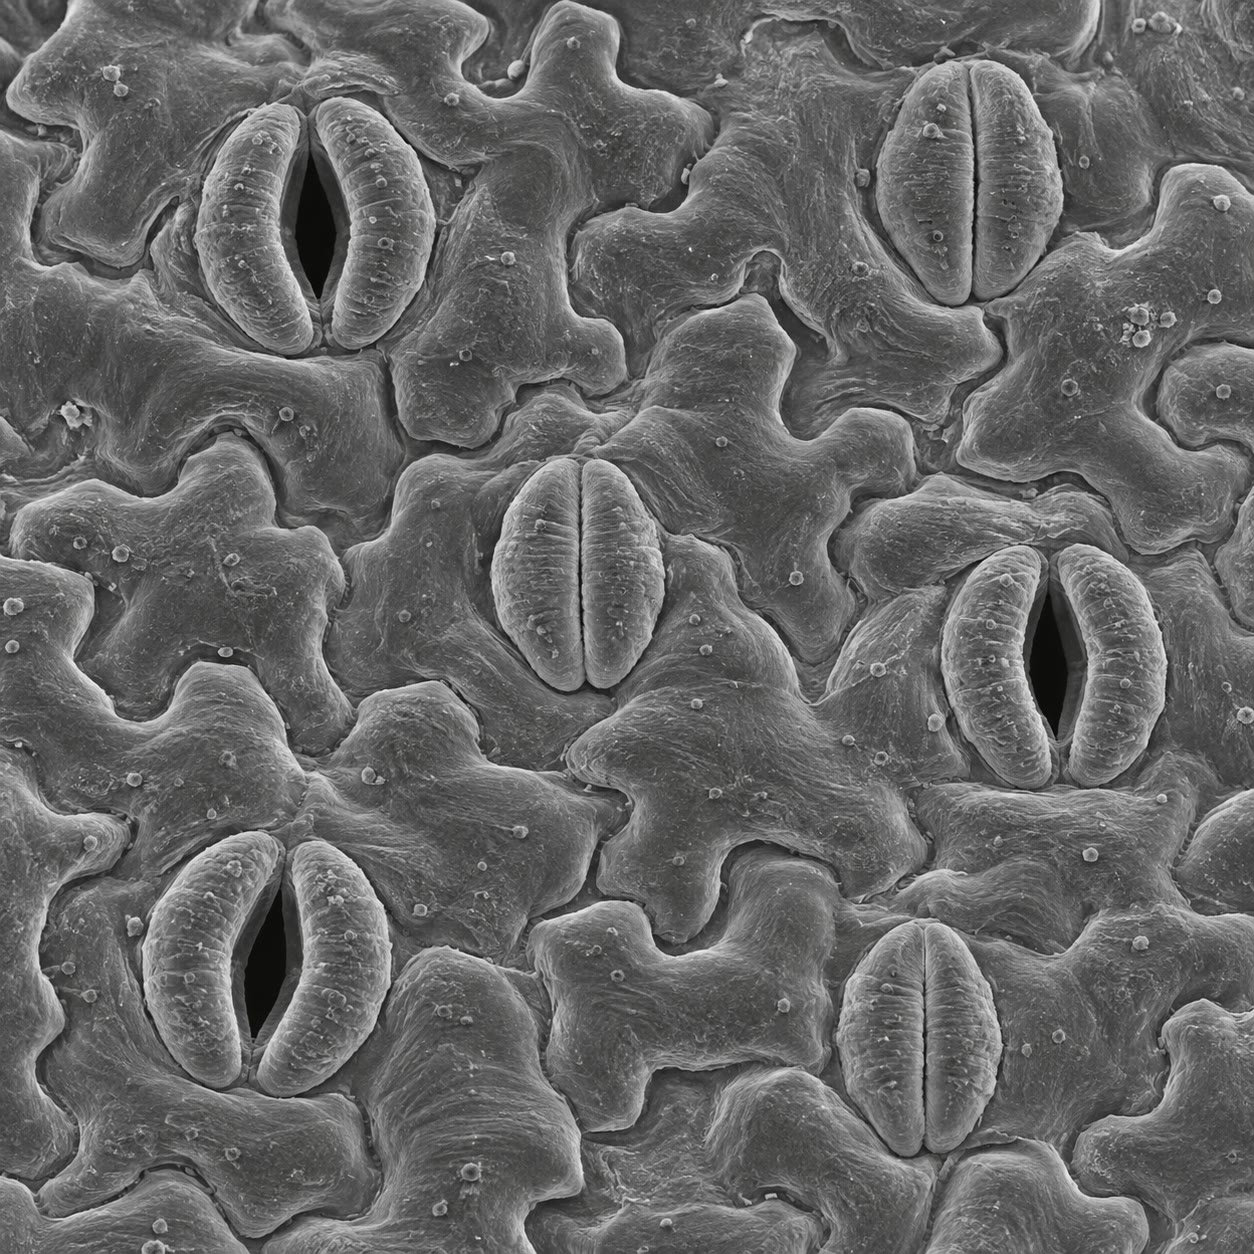
\includegraphics[width=0.42\linewidth]{images/book4/ai/b4-15-stomata-sem.jpg}

{\small Stoma pada sisi bawah sehelai daun, sebagian membuka dan
sebagian menutup: dua \omterm{prop:b2:plant-plasticity:stomata}{sel penjaga} mengelilingi tiap porinya, katup yang
dengannya daunnya menukar air dengan karbon dioksida.}
\end{omfigure}

\begin{example}[Ongkos karbon sehari]\label{ex:b2:plant-plasticity:wue}
Pada tengah hari sehelai daun bunga matahari dengan $g_s = \qty{0.3}{mol.m^{-2}.s^{-1}}$,
$w_i - w_a = 0.02$, dan $c_a - c_i = \qty{120}{\micro mol/mol}$
bertranspirasi $E = \qty{6}{mmol.m^{-2}.s^{-1}}$ dan memfiksasi $A =
0.3\times 120/1.6 = \qty{22}{\micro mol.m^{-2}.s^{-1}}$: $A/E =
\qty{3.7e-3}{}$, yakni 270 molekul air bagi tiap atom karbon,
\qty{400}{g} air tiap gram karbon. Satu hektar daun semacam itu
kehilangan \qty{40}{t} air pada sebuah hari musim panas untuk
memfiksasi \qty{100}{kg} karbon. Ketika tanahnya mengering, \omterm{def:b2:plant-flowering:dormancy}{asam
absisat} menutup stomanya hingga sepersepuluh konduktans ini: $E$ turun
sepuluh kali lipat, $A$ kurang dari itu (karena $c_i$ ikut turun), dan
tumbuhannya bertahan hidup dengan menu kelaparan alih-alih mati
kehausan.
\end{example}

\begin{proposition}[Adaptasi terhadap kekeringan]\label{prop:b2:plant-plasticity:xerophytes}
\index{xerofit}\index{tumbuhan CAM}\index{sukulen}
Tumbuhan tempat kering (\emph{xerofit}) memadukan struktur dan siasat
yang terwariskan. Kurangi kehilangannya: kutikula yang tebal, stoma
yang terbenam di dalam lekuk atau di bawah rambut (yang menebalkan
lapisan udara yang tenang), daun yang tereduksi menjadi duri (kaktus)
atau yang digugurkan pada musim kering, daun kecil tebal yang
menggulung. Simpan: batang dan daun sukulen dengan lendir yang menahan
air. Jangkau: akar sedalam \qty{50}{m} (mesquite) atau yang menyebar
tepat di bawah permukaannya untuk menangkap sebuah hujan. Geser:
\omterm{prop:b2:plant-plasticity:xerophytes}{tumbuhan CAM} membuka stomanya pada malam hari, ketika $w_i - w_a$
kecil, memfiksasi $\mathrm{CO_2}$ menjadi asam malat, lalu
memfiksasinya ulang di balik stoma yang tertutup pada siang hari ---
karbon yang sama dengan seperlima airnya. Lolos: tumbuhan setahun gurun
hidup sebagai \omterm{def:b2:angiosperm-reproduction:seed}{biji} selama bertahun-tahun lalu merampungkan sebuah \omterm{def:b2:plant-life-cycles:cycles}{daur
hidup} dalam beberapa pekan setelah hujan. Tahankan: tumbuhan kebangkitan
kehilangan \qty{95}{\%} airnya lalu hidup kembali. Tiap siasatnya
memiliki harga --- CAM lambat, kesukulenan berat, duri tidak dapat
berfotosintesis --- dan tumbuhan yang membayarnya terkalahkan
pertumbuhannya di mana pun air berlimpah.
\end{proposition}

\begin{omfigure}
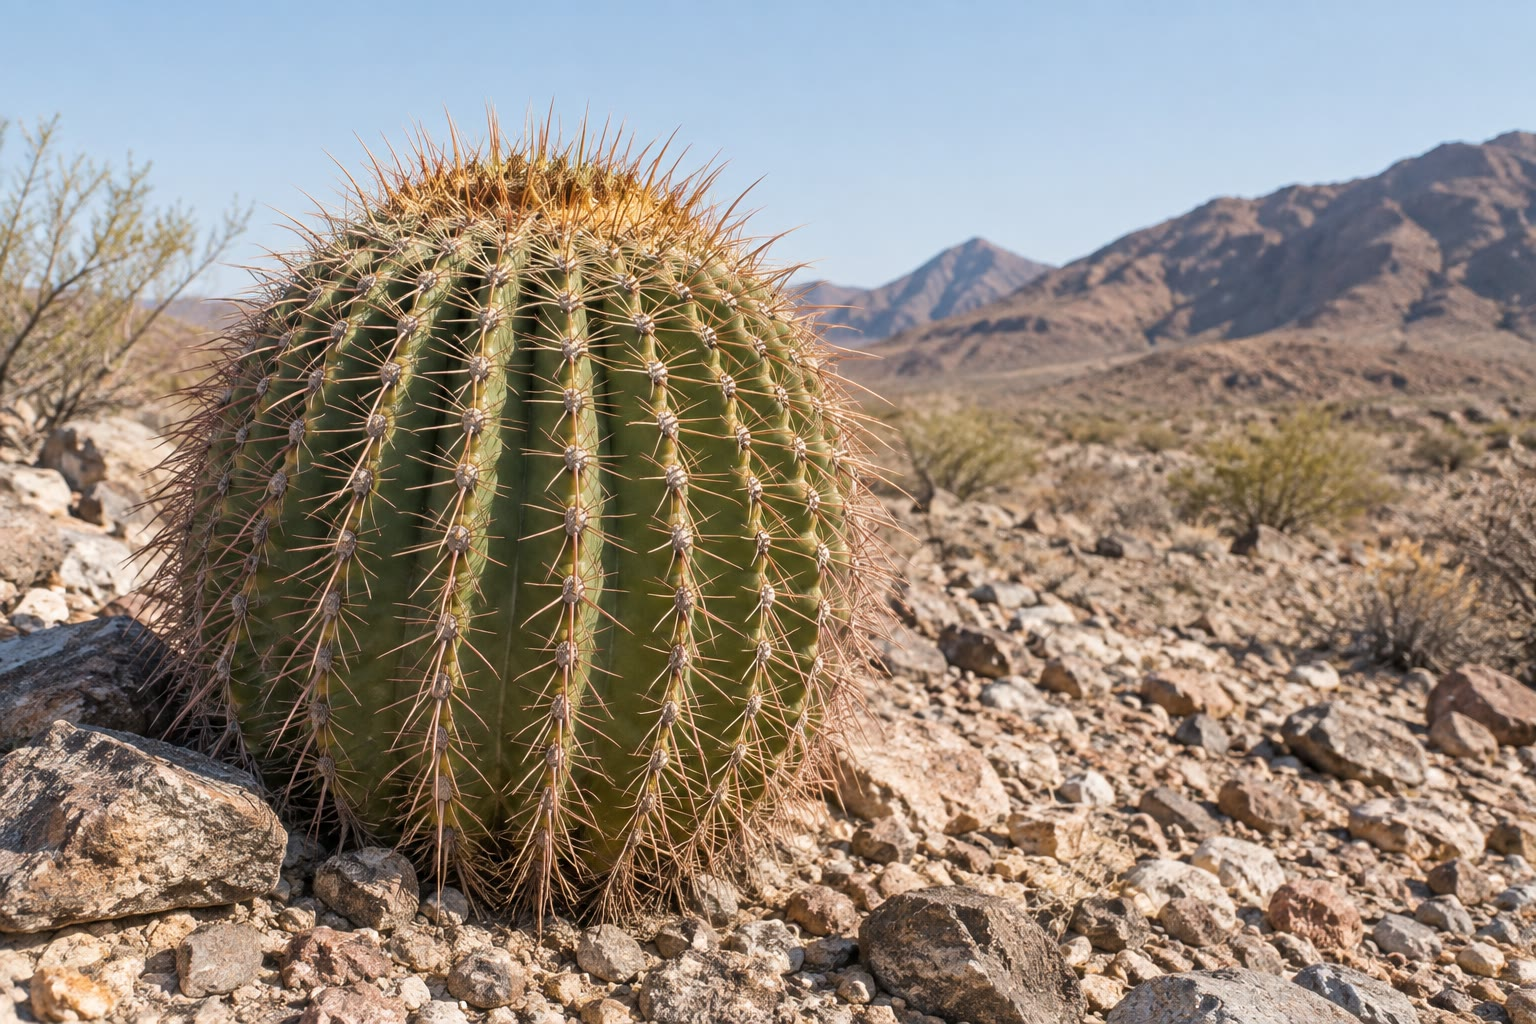
\includegraphics[width=0.55\linewidth]{images/book4/ai/b4-15-cactus.jpg}

{\small Sebatang kaktus tong: batang sukulen dengan kutikula yang
tebal, rusuk yang memungkinkannya menggembung setelah hujan, daun yang
tereduksi menjadi duri, dan stoma yang hanya membuka pada malam hari.}
\end{omfigure}

\section{Dingin, garam, dan tanggapan cekaman}

\begin{proposition}[Aklimasi terhadap cekaman]\label{prop:b2:plant-plasticity:stress}
\index{aklimasi dingin}\index{halofit}\index{protein kejut panas}
Sepekan pada \qty{4}{\celsius} menurunkan suhu yang mematikan sebatang
gandum hitam musim dingin dari \qty{-5}{\celsius} menjadi
\qty{-25}{\celsius}: selnya telah memuati dirinya dengan gula dan
protein yang menurunkan titik bekunya serta melindungi membrannya,
mengubah lipidnya agar tetap encer, dan membuat protein antibeku yang
menghentikan pertumbuhan hablur es; peristiwa yang mematikannya bukan
esnya, yang terbentuk tanpa bahaya di antara sel-selnya, melainkan
dehidrasi selnya ketika airnya keluar untuk bergabung dengan esnya.
Beberapa jam pada \qty{40}{\celsius} mengimbas \emph{\omterm{prop:b2:plant-plasticity:stress}{protein kejut panas}} yang
melipat ulang protein yang terdenaturasi dan melindungi selnya pada
\qty{45}{\celsius}. Garam dihadapi dengan penyingkiran di akarnya,
pemetakan ke dalam vakuolanya (dengan zat terlarut yang serasi di dalam
sitosolnya untuk mengimbanginya), dan, pada \emph{halofit} sejati,
penyekresian lewat kelenjar garam. Sebagian besar tanggapan ini
melewati pensinyalan yang sama: sebuah pengindra, kenaikan kalsium
sitosolnya, \omterm{def:b2:plant-flowering:dormancy}{asam absisat}, dan sekumpulan \omterm{prop:b2:cell-differentiation:transcriptional}{faktor transkripsi} yang
menyalakan ratusan gen pelindung --- sebuah program cekaman yang seumum
tanggapan kebal seekor hewan, dan, seperti tanggapan itu, mahal:
tumbuhan yang beraklimasi tumbuh perlahan, dan tumbuhan yang
beraklimasi ketika ia tidak perlu kalah terhadap tumbuhan yang tidak.
\end{proposition}
\begin{proof}[Bukti eksperimental]
Percobaan \omterm{prop:b2:plant-plasticity:stress}{aklimasi dingin} mengukur suhu yang mematikan separuh sel
sehelai daun (yaitu LT$_{50}$) sebelum dan sesudah sebuah masa pada
suhu rendah; pergeserannya, sebesar sepuluh sampai dua puluh derajat
dalam sepekan, dibalikkan oleh sepekan kehangatan. Mutan yang tidak
mampu menyalakan program dinginnya (yaitu \omterm{prop:b2:cell-differentiation:transcriptional}{faktor transkripsi} CBF)
beraklimasi dengan buruk, dan tumbuhan yang mengungkapkan faktor itu secara
konstitutif bertahan dari embun beku tanpa \omterm{def:b2:plant-plasticity:plasticity}{aklimasi} --- tetapi tumbuh
kerdil.
\end{proof}

\begin{omfigure}
\begin{tikzpicture}[every node/.style={font=\scriptsize}, >=stealth]
  \node[draw, rounded corners, fill=omExo!25, align=center] (s) at (0,0) {cekaman\\kekeringan, dingin,\\garam, panas};
  \node[draw, rounded corners, fill=omDef!15, align=center] (sen) at (3.2,0) {pengindra\\(membran, turgor,\\protein tak terlipat)};
  \node[draw, rounded corners, fill=omDef!15, align=center] (ca) at (6.4,0) {kurir kedua\\Ca$^{2+}$, ABA};
  \node[draw, rounded corners, fill=omProp!20, align=center] (tf) at (9.6,0) {faktor\\transkripsi};
  \node[draw, rounded corners, fill=omThm!15, align=center] (out) at (12.8,0.9) {gen pelindung:\\zat terlarut, antibeku,\\pendamping, pengangkut};
  \node[draw, rounded corners, fill=omThm!15, align=center] (out2) at (12.8,-0.9) {pertumbuhan melambat:\\ongkosnya};
  \draw[->, thick] (s) -- (sen); \draw[->, thick] (sen) -- (ca); \draw[->, thick] (ca) -- (tf);
  \draw[->, thick] (tf) -- (out); \draw[->, thick] (tf) -- (out2);
\end{tikzpicture}

{\small Bentuk umum tanggapan cekaman sebatang tumbuhan: sebuah
pengindra, sebuah isyarat kalsium dan \omterm{def:b2:plant-flowering:dormancy}{asam absisat}, \omterm{prop:b2:cell-differentiation:transcriptional}{faktor
transkripsi}, dan sebuah program gen pelindung --- yang dibayar dengan
pertumbuhan.}
\end{omfigure}

\begin{example}[Isyarat yang berdusta]\label{ex:b2:plant-plasticity:lie}
Keplastisan hanya sebaik isyaratnya. Sebuah semai di bawah naungan
merah jauh tetangganya memanjang --- dengan benar, jika tetangganya
sebuah semai yang dapat ia lampaui; dengan fatal, jika tetangganya
sebatang pohon, karena cadangan yang dibelanjakan untuk batangnya
hilang bagi akar dan daunnya. Tanaman yang ditanam rapat saling
menaungi, memanjang, lalu rebah; pemulia telah menyeleksi gandum dan
padi yang mengabaikan isyarat merah jauhnya. Sepekan yang hangat pada
bulan Februari memunculkan daun yang dibunuh embun beku bulan Maret;
tumbuhan yang bertahan adalah tumbuhan yang juga menghitung dinginnya
(\cref{ch:b2:plant-flowering}). Tiap tanggapan yang plastis adalah
sebuah taruhan atas kejujuran isyaratnya, dan \omterm{def:b2:plant-plasticity:plasticity}{norma reaksinya} dibentuk
oleh seberapa sering, pada masa lalu garis keturunannya, isyaratnya
mengatakan yang sebenarnya.
\end{example}

\section{Latihan}

\begin{exercise}[$\star$]\label{exo:b2:plant-plasticity:1}
Definisikan \omterm{def:b2:plant-plasticity:plasticity}{keplastisan fenotipe}, \omterm{def:b2:plant-plasticity:plasticity}{norma reaksi}, \omterm{def:b2:plant-plasticity:plasticity}{aklimasi}, dan \omterm{def:b2:plant-plasticity:plasticity}{adaptasi},
beserta sebuah contoh tumbuhan bagi masing-masingnya.
\end{exercise}

\begin{exercise}[$\star$]\label{exo:b2:plant-plasticity:2}
Uraikan keempat perlakuan koleoptil Darwin dan apa yang ditunjukkan oleh masing-masingnya.
\end{exercise}

\begin{exercise}[$\star$]\label{exo:b2:plant-plasticity:3}
Sebutkan lima perbedaan antara sehelai \omterm{prop:b2:plant-plasticity:sunshade}{daun matahari} dan sehelai \omterm{prop:b2:plant-plasticity:sunshade}{daun
naungan}, dan katakan kapan dalam hidup daunnya pilihannya diambil.
\end{exercise}

\begin{exercise}[$\star$]\label{exo:b2:plant-plasticity:4}
Bagaimana sebuah stoma membuka, apa yang membukanya pada pagi hari, dan
apa yang menutupnya pada sebuah kekeringan?
\end{exercise}

\begin{exercise}[$\star\star$]\label{exo:b2:plant-plasticity:5}
Hitunglah $\varphi$ bagi $R{:}FR = 1.15$ (matahari), $0.7$ (sebuah
rumpang), $0.2$ (di bawah sebuah kanopi), dan $0.05$ (naungan yang
dalam) dengan $a = 0.77$. Di antara dua yang manakah tumbuhannya
menyalakan \omterm{thm:b2:plant-plasticity:phytochrome}{penghindaran naungan} jika ambangnya $\varphi = 0.4$?
\end{exercise}

\begin{exercise}[$\star\star$]\label{exo:b2:plant-plasticity:6}
Sehelai daun memiliki $g_s = \qty{0.25}{mol.m^{-2}.s^{-1}}$, $w_i - w_a = 0.025$,
$c_a - c_i = \qty{100}{\micro mol/mol}$. Hitunglah $E$, $A$, daya guna
pemakaian airnya dalam mol dan dalam gram air tiap gram karbon, serta
air yang hilang tiap meter persegi dalam sehari selama 12 jam.
\end{exercise}

\begin{exercise}[$\star\star$]\label{exo:b2:plant-plasticity:7}
Hitung ulang latihan sebelumnya bagi sebatang \omterm{prop:b2:plant-plasticity:xerophytes}{tumbuhan CAM} yang
stomanya membuka pada malam hari dengan $w_i - w_a = 0.005$ dan
konduktans yang sama. Dengan faktor berapa ongkos air karbonnya turun?
\end{exercise}

\begin{exercise}[$\star\star$]\label{exo:b2:plant-plasticity:8}
Sebuah statolit adalah butir pati berjari-jari \qty{2}{\micro m} dengan
rapat massa \qty{1500}{kg/m^3} di dalam sitoplasma yang rapat massanya
\qty{1100}{kg/m^3} dan kekentalannya \qty{0.01}{Pa.s}. Hitunglah laju
endapnya (Stokes) dan waktu untuk melintasi sebuah sel
\qty{10}{\micro m}. Mengapa sebuah klinostat yang berputar sekali tiap
menit meniadakan gravitropismenya?
\end{exercise}

\begin{exercise}[$\star\star$]\label{exo:b2:plant-plasticity:9}
Sebatang batang bergaris tengah \qty{2}{mm} tumbuh \qty{2}{\%} tiap jam
sepanjang sebuah zona \qty{20}{mm}. Cahaya dari satu sisi membagi
auksinnya $60 : 40$. Melalui sudut berapa ia telah membengkok setelah
dua jam? Setelah berapa lama ia berada pada \qty{90}{\degree} terhadap arah asalnya?
\end{exercise}

\begin{exercise}[$\star\star\star$]\label{exo:b2:plant-plasticity:10}
Sebuah semai dengan cadangan \qty{50}{mg} memanjang \qty{2}{cm} sehari
di tempat terbuka dan \qty{4}{cm} sehari di bawah sebuah kanopi, dengan
membelanjakan cadangan \qty{1}{mg} tiap sentimeter batangnya melampaui
apa yang dipasok daunnya. Kanopinya berada \qty{30}{cm} di atasnya pada
sebuah rumpun jelatang dan \qty{10}{m} di dalam sebuah hutan. Pada
keadaan yang manakah \omterm{thm:b2:plant-plasticity:phytochrome}{penghindaran naungannya} berhasil, dan apa yang terjadi pada keadaan yang lain?
\end{exercise}

\begin{exercise}[$\star\star\star$]\label{exo:b2:plant-plasticity:11}
Jelaskan mengapa pembekuan membunuh sebuah sel lewat dehidrasi dan
bukan lewat esnya, apa yang dikerjakan sepekan dingin untuk
mencegahnya, dan mengapa tumbuhan yang mengungkapkan program dinginnya
sepanjang tahun menjadi kerdil.
\end{exercise}

\begin{exercise}[$\star\star\star$]\label{exo:b2:plant-plasticity:12}
``Keplastisan adalah sebuah taruhan atas kejujuran sebuah isyarat.''
Bahaslah dengan isyarat merah jauhnya, sepekan yang hangat pada bulan
Februari, dan pemuliaan tanaman yang mengabaikan tetangganya.
\end{exercise}

\section{Soal: Sebuah Semai di Bawah Kanopi}

\begin{problem}[{Soal akhir pekan --- iklim cahaya, pemanjangan,
anggaran air, dan tropisme sebuah semai dihitung dari fisika
pengindranya, berakhir pada keadaan fitokromnya, tingginya setelah dua
pekan, dan pemakaian air hariannya}]
\label{pb:b2:plant-plasticity:1}
Sebuah semai birch berkecambah di bawah sebuah kanopi yang meneruskan
\qty{3}{\%} cahaya mataharinya dan menurunkan $R{:}FR$ dari $1.15$
menjadi $0.2$ ($a = 0.77$). Di bawah matahari penuh ia akan memanjang
\qty{1.5}{cm} sehari; di bawah kanopinya laju pemanjangannya dikalikan
$1 +
2(0.6 - \varphi)$. Batangnya bergaris tengah \qty{2}{mm} dengan zona
tumbuh \qty{15}{mm}. Daunnya: \qty{20}{cm^2} seluruhnya; $g_s =
\qty{0.2}{mol.m^{-2}.s^{-1}}$; $w_i - w_a = 0.015$ di dalam
naungannya, $0.03$ di dalam sebuah rumpang; $c_a - c_i = \qty{80}{\micro mol/mol}$;
harinya berlangsung \qty{14}{h}. Statolitnya: jari-jari \qty{2.5}{\micro m},
rapat massa \qty{1500}{kg/m^3}, di dalam sitoplasma \qty{1100}{kg/m^3}
dan \qty{0.01}{Pa.s}.

\medskip
\noindent\textbf{Bagian I --- Cahayanya.}
\begin{enumerate}
  \item Hitunglah $\varphi$ di tempat terbuka dan di bawah kanopinya.
  \item Apa yang disimpulkan semainya dari $\varphi$, dan apa yang
        akan ia simpulkan jika kanopinya meneruskan \qty{3}{\%}
        cahayanya tanpa mengubah warnanya (sebuah kain naung)?
  \item Hitunglah laju pemanjangannya di bawah kanopinya.
  \item Seberapa tinggi semainya setelah 14 hari di sana, terhadap
        seorang saudaranya di tempat terbuka?
  \item Sebuah rumpang terbuka pada satu sisi, menaikkan $R{:}FR$ pada
        sisi itu menjadi $0.8$. Dua tanggapan apa yang menyusul, dan
        lewat dua fotoreseptor yang mana?
  \item Mengapa daun yang dikembangkan di bawah kanopi lebih lebar dan
        lebih tipis, dan apa yang terjadi padanya jika kanopinya ditebang?
\end{enumerate}

\medskip
\noindent\textbf{Bagian II --- Membengkok menuju rumpangnya.}
\begin{enumerate}[resume]
  \item Cahaya dari rumpangnya membagi auksinnya $65 : 35$ melintasi
        batangnya. Dengan laju pemanjangan di bawah kanopi pada
        pertanyaan 3, hitunglah pemanjangan nisbi tiap sisi zona
        tumbuhnya dalam satu jam.
  \item Hitunglah sudut pembengkokannya setelah satu jam.
  \item Setelah berapa lama batangnya menunjuk lurus ke rumpangnya,
        jika rumpangnya berada pada \qty{60}{\degree} dari tegak?
  \item Batangnya kini condong. Hitunglah laju endap sebuah statolit
        dan waktu untuk melintasi sebuah sel \qty{12}{\micro m}.
  \item Gravitropisme pucuknya dan fototropismenya kini berselisih.
        Mana yang menang pada tumbuhan yang menghindari naungan, dan
        mengapa hal itu adaptif?
  \item Sebuah akar semai yang sama dimiringkan \qty{45}{\degree} oleh
        sebuah batu. Ramalkan tanggapannya dan jelaskan mengapa
        tanggapannya berlawanan dengan tanggapan pucuknya walaupun
        mekanismenya sama.
\end{enumerate}

\medskip
\noindent\textbf{Bagian III --- Airnya.}
\begin{enumerate}[resume]
  \item Hitunglah laju transpirasi tiap meter persegi di dalam
        naungannya, dan air yang hilang oleh daun semainya dalam sehari.
  \item Hitunglah karbon yang difiksasi tiap meter persegi tiap detik
        dan tiap hari, serta daya guna pemakaian airnya dalam gram air
        tiap gram karbon.
  \item Berapakah perolehan karbon harian seluruh semainya di dalam
        naungannya, dalam miligram?
  \item Hitung ulang air yang hilang dan daya gunanya di dalam
        rumpangnya.
  \item Tanahnya mengering dan \omterm{def:b2:plant-flowering:dormancy}{asam absisat} menurunkan $g_s$ menjadi
        \qty{0.02}{mol.m^{-2}.s^{-1}}. Hitung ulang $E$ dan $A$
        (anggaplah $c_a - c_i$ naik menjadi \qty{200}{\micro mol/mol}).
        Mana yang turun lebih banyak, dan mengapa?
  \item Semainya memiliki \qty{5}{g} jaringan daun yang \qty{85}{\%}
        berupa air dan dapat kehilangan seperlimanya sebelum layu.
        Berapa lama ia bertahan di dalam rumpangnya dengan stoma yang
        terbuka jika akarnya tidak memasok apa pun?
  \item Jelaskan mengapa siasat CAM tidak akan cocok bagi sebuah semai
        birch di bawah sebuah kanopi.
\end{enumerate}

\medskip
\noindent\textbf{Bagian IV --- Taruhannya.}
\begin{enumerate}[resume]
  \item Semainya menyimpan cadangan \qty{100}{mg} dan membelanjakan
        \qty{2}{mg} tiap sentimeter batangnya melampaui apa yang
        dipasok daunnya di dalam naungannya. Seberapa banyak batang
        yang dapat ia bangun dengan cadangannya saja?
  \item Kanopinya adalah sebuah rumpun jelatang \qty{40}{cm} di
        atasnya; lalu sebuah hutan \qty{8}{m} di atasnya. Katakan pada
        tiap keadaan apakah pemanjangannya mencapai cahaya sebelum
        cadangannya habis, dan tanggapan apa yang akan lebih baik di
        dalam hutannya.
  \item Sebatang birch adalah perintis tanah terbuka; sebuah semai
        beech dapat menunggu berpuluh tahun di dalam naungan yang
        dalam. Bandingkan \omterm{def:b2:plant-plasticity:plasticity}{norma reaksi} yang diharapkan dari keduanya
        terhadap $\varphi$.
  \item Seorang pemulia tanaman menginginkan tanaman yang ditanam
        rapat yang tidak memanjang. Pengindra atau tanggapan yang mana
        yang akan Anda lumpuhkan, dan efek samping apa yang harus Anda
        periksa?
  \item Jelaskan dalam dua kalimat mengapa tumbuhan yang tidak dapat
        mengindra tetangganya dan tumbuhan yang selalu memercayainya
        sama-sama lebih buruk nasibnya daripada tumbuhan yang
        kadang-kadang memercayainya.
  \item Nyatakan hasilnya: $\varphi$ di bawah matahari dan di dalam
        naungan, tinggi semainya setelah 14 hari, dan pemakaian air
        hariannya di dalam naungan dan di dalam rumpangnya.
\end{enumerate}
\end{problem}
